\subsection{SPMD sum}

The \definition{Single Program Multiple Data (SPMD)} is a term that has been used to \textbf{describe computational models} for exploiting parallelism, where \textbf{multiple processors work together to execute a program to get results faster}.

\highspace
In this section, we will see an SPMD approach on a Parallel Random Access Machine (PRAM). We will introduce one of the most common and simple mathematical operations: the sum.

\highspace
The following pseudocode takes as \textbf{input an array} of size $n = 2^{k}$. In this case, $n$ is a power of 2 because it ensures that the array can be evenly divided at each step of the computation. The value $k$ is the number of iterations or levels of the summation process.
\begin{lstlisting}[mathescape=true, caption={Single Program Multiple Data (SPMD) sum}]
BEGIN
    GLOBAL READ (A $\leftarrow$ A(I))
    GLOBAL WRITE (A $\rightarrow$ B(I))
    FOR H = 1 : K
        IF $i \le n \div 2^{h}$ THEN BEGIN
            GLOBAL READ (X $\leftarrow$ B(2$i$ - 1))
            GLOBAL READ (Y $\leftarrow$ B(2$i$))
            Z := X + Y
            GLOBAL WRITE (Z $\rightarrow$ B($i$))
        END
    IF I = 1 THEN
        GLOBAL WRITE (Z $\rightarrow$ S)
END
\end{lstlisting}
\begin{itemize}
    \item First, read the entire input array \texttt{A} and copy the read data to another array \texttt{B}.
    
    \item Loop over \texttt{h} (\texttt{1 to k}). In each iteration, for each index $i$ less than or equal to $n \div 2^{h}$, read values from array \texttt{B} at positions $2i-1$ and $2i$; sum these values (and store the result in \texttt{Z}) and store the result (\texttt{Z}) back into \texttt{B($i$)}.
    
    \item Once all iterations are complete, the final sum is stored in a variable \texttt{S}.
\end{itemize}
For example, if $n = 8$, then $k$ would be 3, meaning that the algorithm will run for 3 iterations to sum all the elements in parallel.
\begin{table}[!htp]
    \centering
    \begin{tabular}{@{} c c c @{}}
        \toprule
        $h$ & $i$ & adding \\
        \midrule
        \multirow{4}{*}{1} & 1 & 1,2 \\
          & 2 & 3,4 \\
          & 3 & 5,6 \\
          & 4 & 7,8 \\
        \cmidrule{1-3}
        \multirow{2}{*}{2} & 1 & 1,2 \\
          & 2 & 3,4 \\
        \cmidrule{1-3}
        3 & 1 & 1,2 \\
        \bottomrule
    \end{tabular}
\end{table}

\newpage

\begin{figure}[!htp]
    \centering
    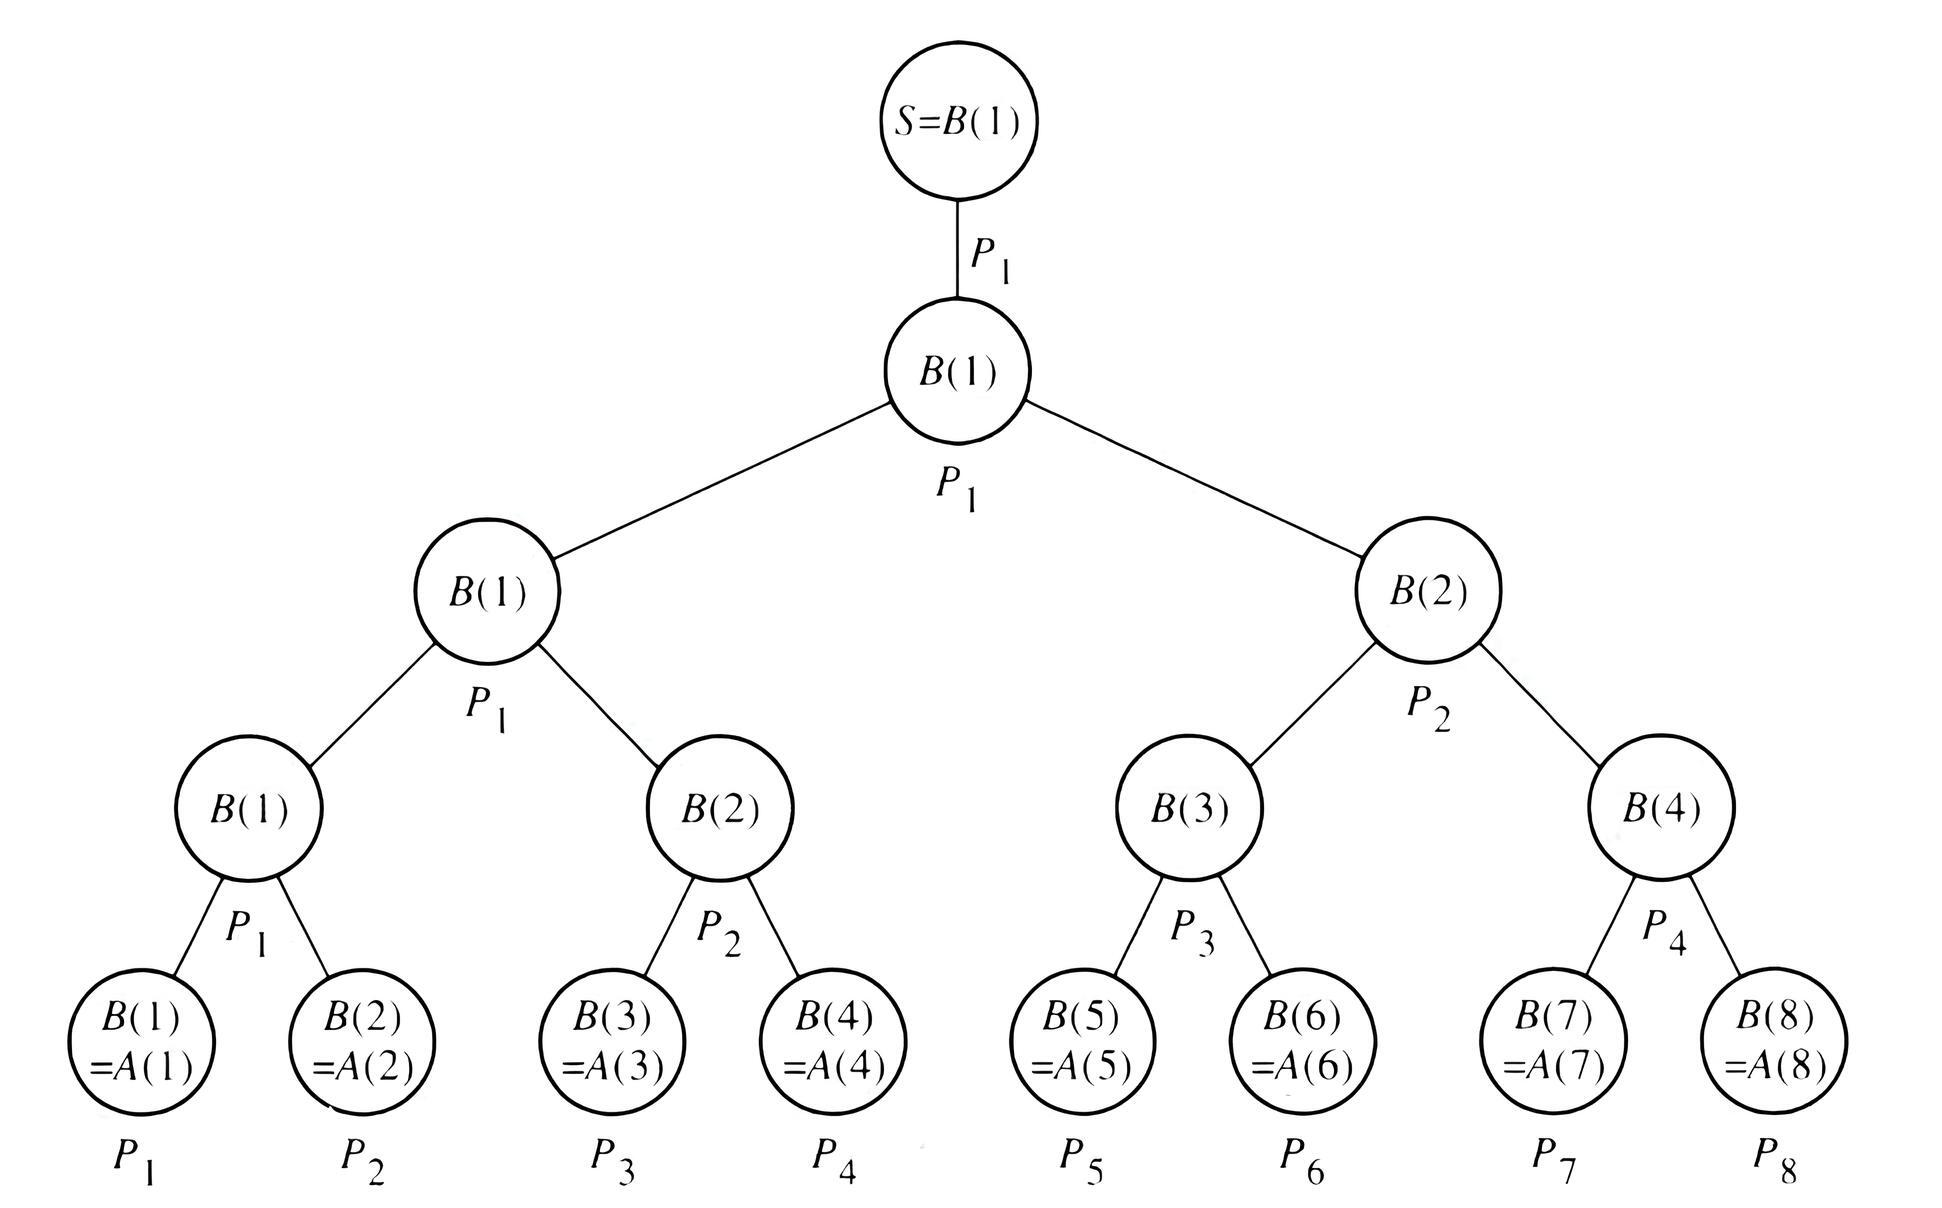
\includegraphics[width=\textwidth]{img/SPDM-sum-1.jpg}
    \caption{Computation of the sum of eight elements on a PRAM with eight processors. Each internal node represents a sum operation. The specific processor executing the operation is indicated below each node.}
    \label{fig: SPDM-sum-1}
\end{figure}

\begin{flushleft}
    \textcolor{Green3}{\faIcon{tachometer-alt} \textbf{Performance of sum}}
\end{flushleft}
When the size of the array is equal to the number of processors ($N = P$), the \textbf{speedup and efficiency decrease}:
\begin{itemize}
    \item $T^{*}\left(N\right) = T_{1}\left(N\right) = N$
    \item $T_{N=P}\left(N\right) = 2 + \log N$
    \item $\mathrm{SU}_{P} = \dfrac{N}{2+\log N}$
    \item $T^{*}\left(N\right) = P \cdot \left(2 + \log N\right) \approx N \log N$
    \item $E_{p} = \dfrac{T_{1}}{pT_{p}} = \dfrac{N}{N \log N} = \dfrac{1}{\log N}$
\end{itemize}
\begin{figure}[!htp]
    \centering
    \begin{subfigure}[h]{0.45\linewidth}
        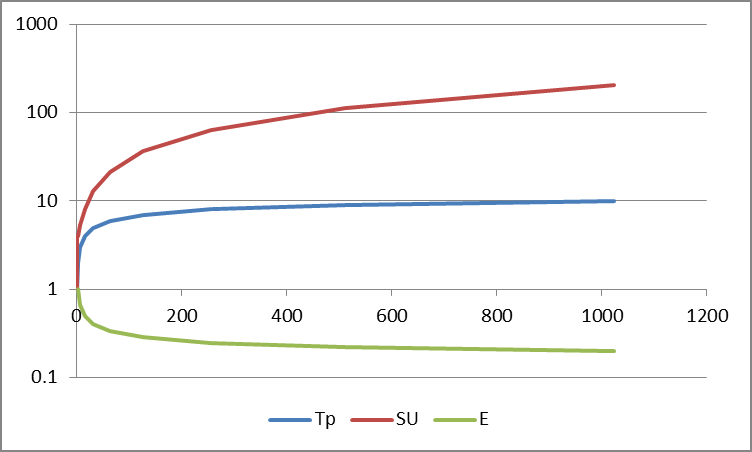
\includegraphics[width=\linewidth]{img/SPDM-sum-2.png}
    \end{subfigure}
    \hfill
    \begin{subfigure}[h]{0.45\linewidth}
        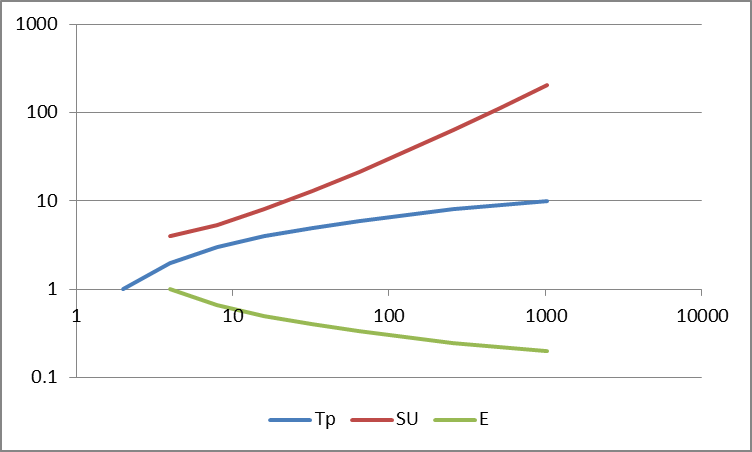
\includegraphics[width=\linewidth]{img/SPDM-sum-3.png}
    \end{subfigure}
\end{figure}

\newpage

\noindent
If the size of the array is much larger than the number of processors ($N \gg P$), the \textbf{speedup and power are linear}, the \textbf{cost is fixed} and the \textbf{efficiency is maximum (equal to 1)}:
\begin{itemize}
    \item $T^{*}\left(N\right) = T_{1}\left(N\right) = N$
    \item $T_{p}\left(N\right) = \dfrac{N}{p} + \log p$
    \item $\mathrm{SU}_{P} = \dfrac{N}{\frac{N}{p}+\log p} \approx P$
    \item $\text{COST} = p\left(\dfrac{N}{p} + \log p\right) \approx N$
    \item $\text{WORK} = N + P \approx N$
    \item $E_{p} = \dfrac{T_{1}}{pT_{p}} = \dfrac{N}{p\left(\frac{N}{p} + \log p\right)} \approx 1$
\end{itemize}
\begin{figure}[!htp]
    \centering
    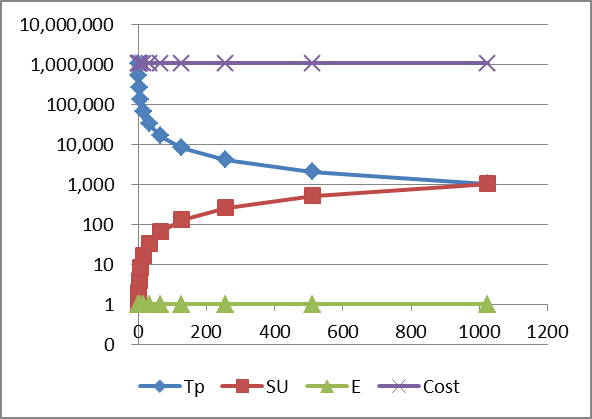
\includegraphics[width=.5\linewidth]{img/SPDM-sum-4.png}
    \caption*{$n = 1'000'000$}
\end{figure}

\begin{examplebox}
    Refer to Figure \ref{fig: SPDM-sum-1} (page \pageref{fig: SPDM-sum-1}), the performance metrics are:
    \begin{itemize}
        \item $T_{8} = 5$
        \item $C = 8 \cdot 5 = 40$ (could do 40 steps)
        \item $W = 2n = 16$ (16 on 40, wasted 24)
        \item $E_{p} = \dfrac{2}{\log n} = \dfrac{2}{3} = 0.67$
        \item $\dfrac{W}{C} = \dfrac{16}{40} = 0.4$
    \end{itemize}
\end{examplebox}